\documentclass[11pt, oneside]{article} 
\usepackage{geometry}
\geometry{letterpaper} 
\usepackage{graphicx}
	
\usepackage{amssymb}
\usepackage{amsmath}
\usepackage{parskip}
\usepackage{color}
\usepackage{hyperref}

\graphicspath{{/Users/telliott_admin/Dropbox/Tex/png/}}
% \begin{center} 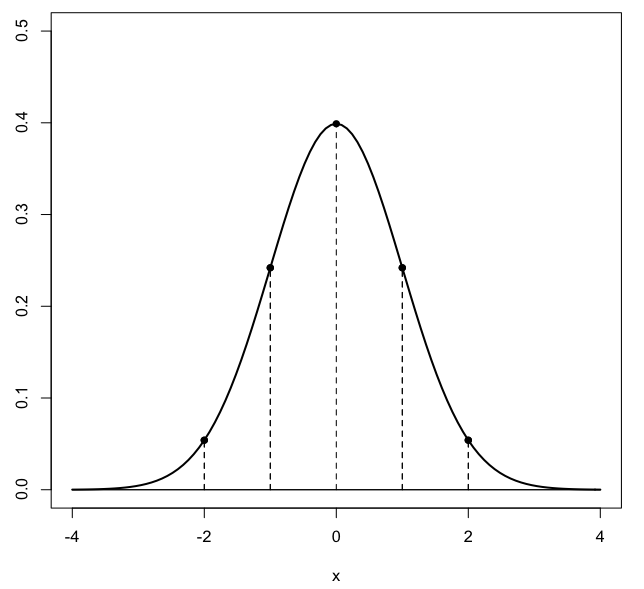
\includegraphics [scale=0.4] {gauss3.png} \end{center}

\title{Distance}
\date{}

\begin{document}
\maketitle
\Large
\subsection*{inequalities}
For any two numbers $a < b$ it is also true that $-b < -a$.  Multiplication by $-1$ switches the direction of the inequality.

$\bullet$  Proof:  add $-a -b$ to both sides above.

We define $x < 0$ below as follows:  first define $m > 0$ and then let $x = -m$.
\subsection*{Absolute value function}
If $x \ge 0$ then $|x| = x$.

For $x < 0$:   $|x| = |-m| = m$.

The following theorem involves a given constant real number $a > 0$ and a real number $x$.
\subsection*{Theorem}
$-a < x < a \Rightarrow |x| < a$.

$\bullet$  Proof:

$\circ$  $x \ge 0$, then $|x| = x$.  We are given $x < a$ $\Rightarrow$ $|x| < a$.

$\circ$  $ x < 0$, then $|x| = m$.  We are given $x > -a$, $-m > -a$, $m < a$ $\Rightarrow$ $|x| < a$.
\subsection*{Theorem}
$|x| < a  \Rightarrow -a < x < a$.

$\bullet$  Proof:

$\circ$  $x \ge 0$, and we are given $|x| < a$.  Since $|x| = x$, we have $x < a$.  Also, since $0 \le x$ and $-a < 0$, we have $-a < x$.  Hence $-a < x < a$.

$\circ$  $x < 0$, then certainly $x < a$.  Since $|x| = m$, that implies $m < a$, so $-x < a$ and therefore $-a < x$.  Hence $-a < x < a$.

We have shown that $-a < x < a \iff |x| < a$.  This completes the proof of the theorem.

\subsection*{Theorem}
Consider a point $p$ in the middle of an interval of length $2 \delta$ so $I = [p - \delta, p + \delta]$.

In other words, $p - \delta < x < p + \delta$ implies that $- \delta < x - p < \delta$ but by the theorem above, this is true $\iff |x-p| < \delta$.

\end{document}}